% XCircuit output "pd.tex" for LaTeX input from pd.eps
\def\putbox#1#2#3#4{\makebox[0in][l]{\makebox[#1][l]{}\raisebox{\baselineskip}[0in][0in]{\raisebox{#2}[0in][0in]{\scalebox{#3}{#4}}}}}
\def\rightbox#1{\makebox[0in][r]{#1}}
\def\centbox#1{\makebox[0in]{#1}}
\def\topbox#1{\raisebox{-0.60\baselineskip}[0in][0in]{#1}}
\def\midbox#1{\raisebox{-0.20\baselineskip}[0in][0in]{#1}}
   \scalebox{1}{
   \normalsize
   \parbox{5.25521in}{
   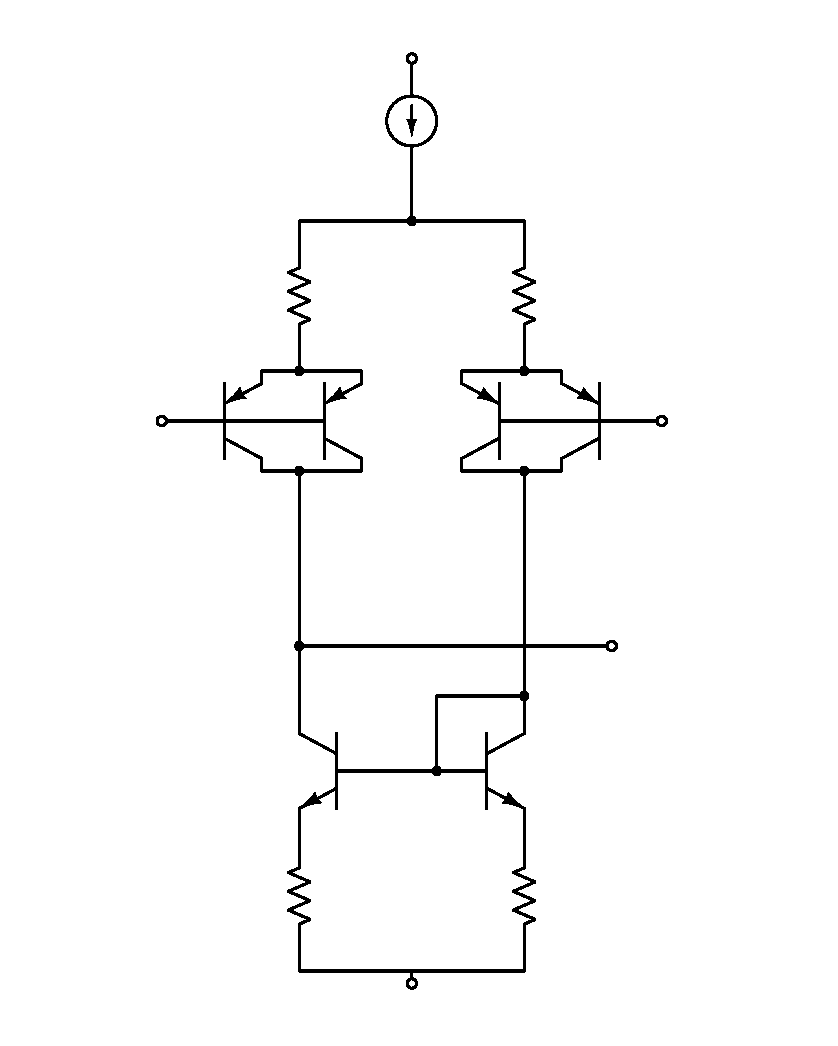
\includegraphics[scale=1]{pd}\\
   % translate x=687 y=960 scale 0.38
   \putbox{2.63in}{6.56in}{1.20}{\centbox{$+V_{CCH}$}}%
   \putbox{2.63in}{0.22in}{1.20}{\centbox{\topbox{$-V_{CCH}$}}}%
   \putbox{0.88in}{4.06in}{1.20}{\rightbox{\midbox{$v_{IN}$}}}%
   \putbox{4.38in}{4.06in}{1.20}{\midbox{$v_{F}$}}%
   \putbox{4.05in}{2.56in}{1.20}{\midbox{$v_{O_{pd}}$}}%
   } % close 'parbox'
   } % close 'scalebox'
   \vspace{-\baselineskip} % this is not necessary, but looks better
